
\renewcommand{\EntradaBibtex}{AplicacionMovilManoRobotica_SistemasInteligentes_UPV_2023}


\begin{frame}{\citetitle{\EntradaBibtex} \footnotemark[1] (1)}
\begin{block}{Propuesta} 
Un modelo 3D dinámico de una Mano controlado por el usuario implementado en un teléfono inteligente
\end{block} 
\begin{itemize}
\item Utiliza la cámara del teléfono inteligente para detectar la mano (Libreria MediaPipe)
\item Utiliza OpenGL ES para crear el entorno 3D de una mano humana modelada en Blender
\item En base a los movimientos de los dedos del usuario, el modelo se actualiza
\end{itemize}
\footnotetext[1]{\fullcite{\EntradaBibtex}}
\end{frame}

\begin{frame}{\citetitle{\EntradaBibtex} (2)}

\begin{center}
	\begin{tabular}{ccc}
		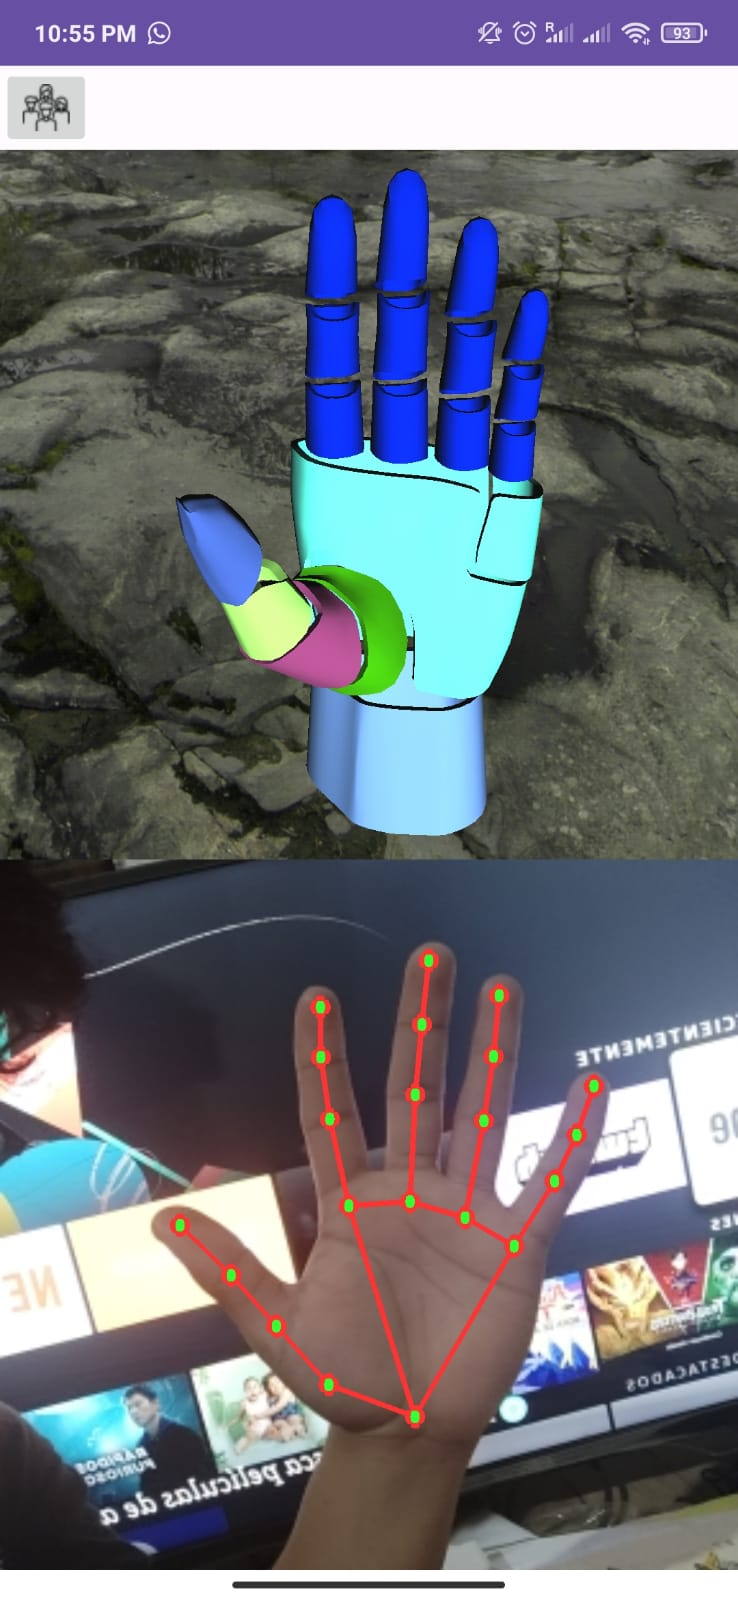
\includegraphics[width=0.20\linewidth]{2023_ManoRobotica/figs/hand01.jpeg} &
		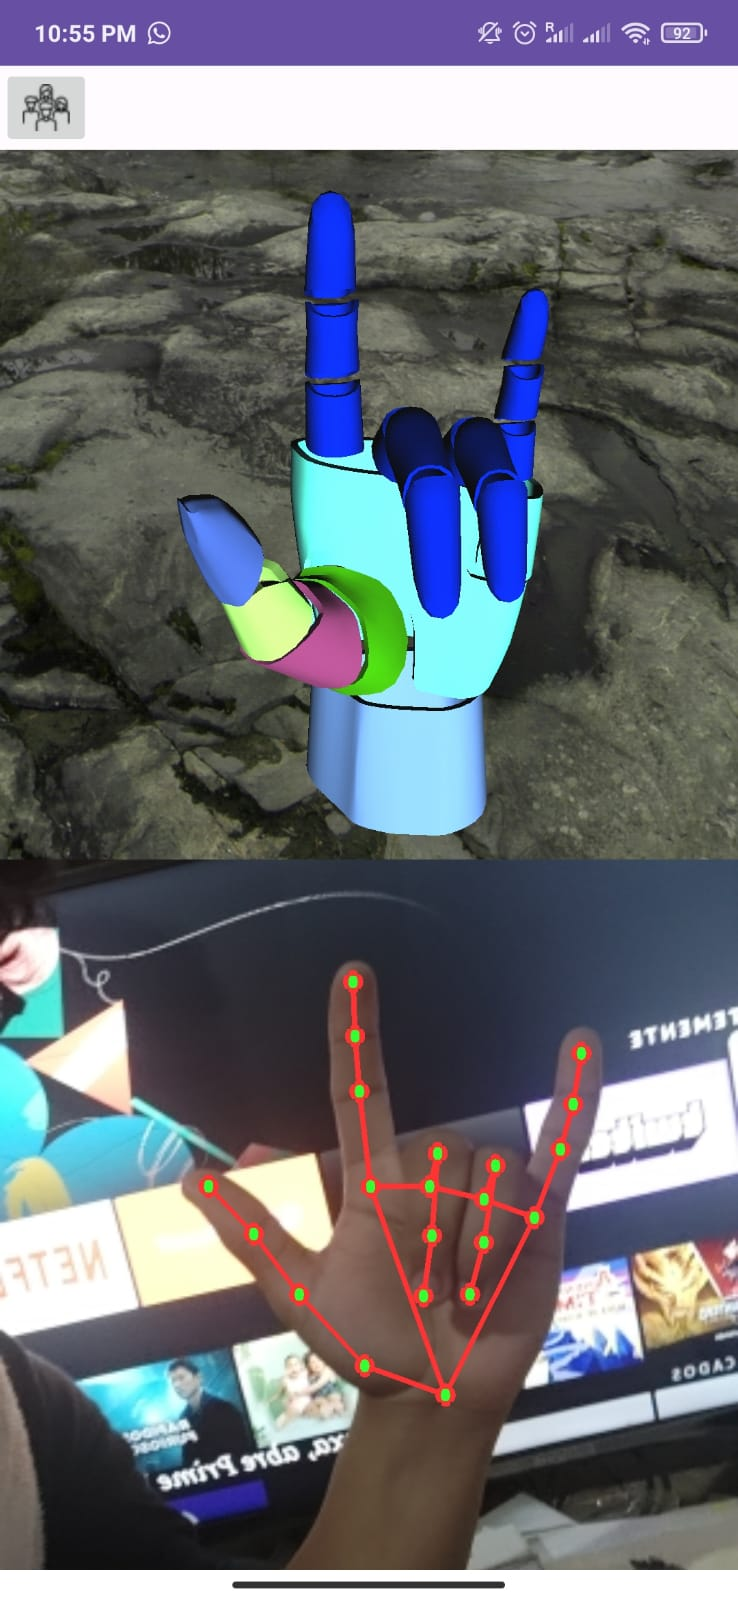
\includegraphics[width=0.20\linewidth]{2023_ManoRobotica/figs/hand02.jpeg} & 
		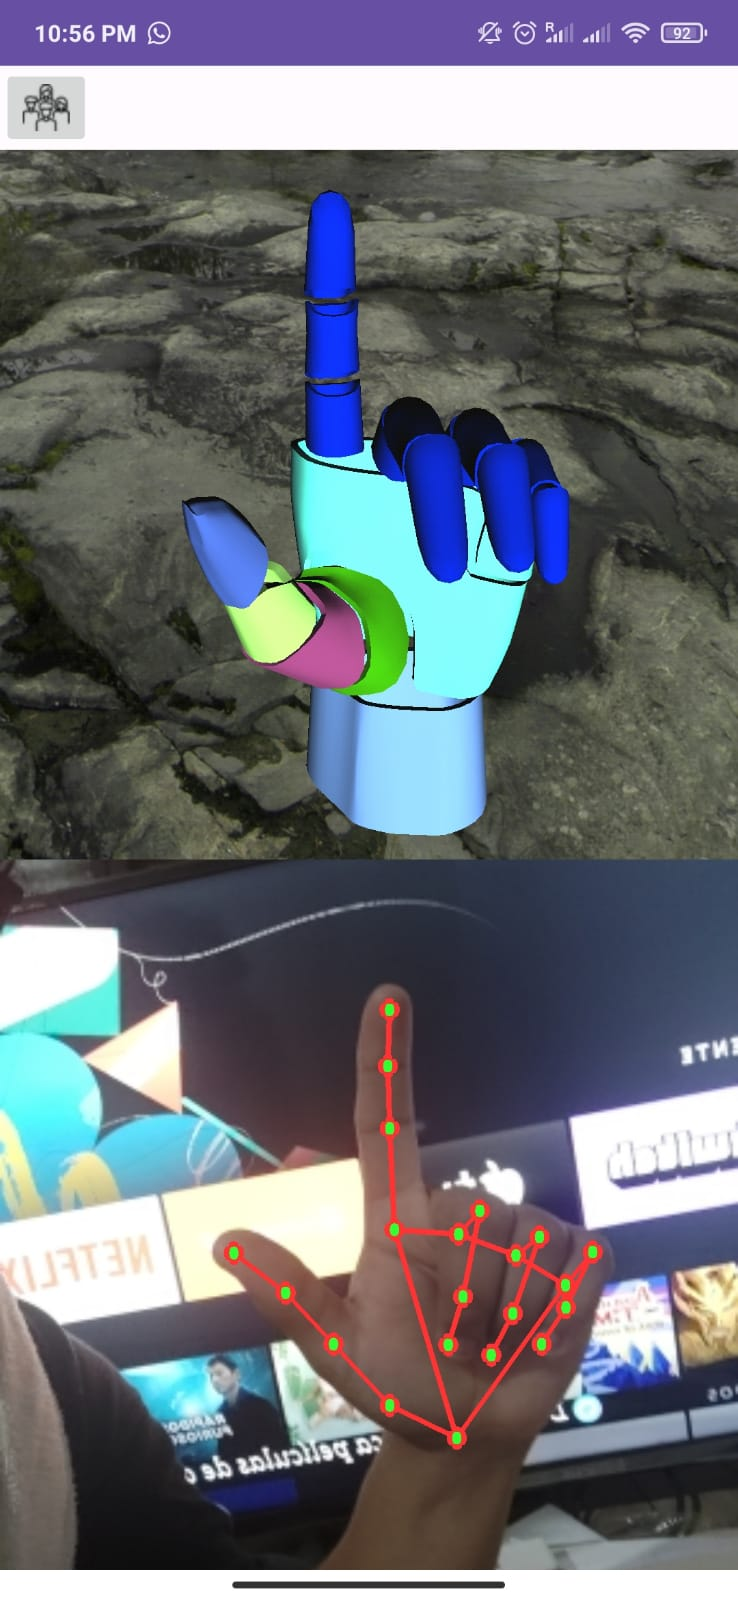
\includegraphics[width=0.20\linewidth]{2023_ManoRobotica/figs/hand03.jpeg}\\
	\end{tabular}
\end{center}

\end{frame}

%


